\section{Results}

Comparison of the splitting method for the repetition code with different code distances and initial Markov chain length $T_{\text{init}}$.
For code distance 5, the logical error rates for one realization of the splitting method for each $T_{\text{init}}\in\{2,4,\ldots,20\}$ are shown in
Fig. \ref{fig:d5_rep_raw}.

\begin{figure}[h]
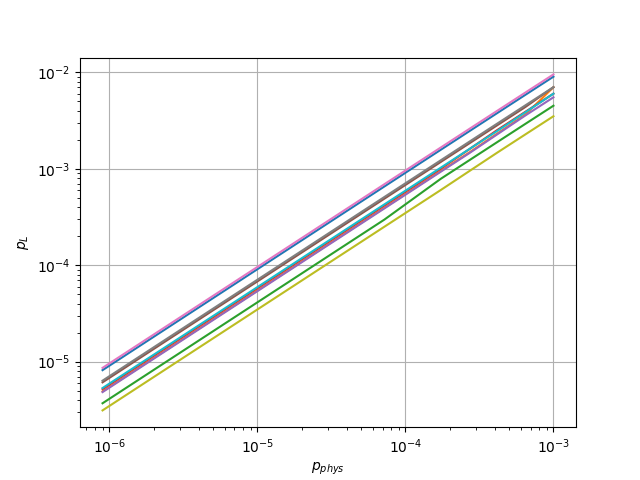
\includegraphics[width=0.8\textwidth]{figs/d5_rep_raw.png} 
\caption{}
\label{fig:d5_rep_raw}
\end{figure}

The difference between realizations can be attributed to different estimations of the initial logical error rate $p_1$, obtained using direct Monte Carlo sampling.
The average and standard deviations of the logical error rates for multiple realizations at each $T_{\text{init}}$, corrected for differences in $p_1$,
is shown in \ref{fig:d5_analysis}(a). The number of times the length of the Markov Chain $T_j$ is updated is shown in (b). 
The total computing time grows linearly with the total length, as we can see in the comparison in (c) between the actual times and the expected times.
The uncertainty of the logical error estimation at the lowest physical error rate is plotted as a function of $T_{\text{init}}$ is plotted in (d).
The uncertainty does not vary significantly as a function of $T_{\text{init}}$.

\begin{figure}[h]

\includegraphics[width=0.8\textwidth]{figs/d5_analysis.png} 
\caption{Analysis for distance 5 repetition code and $T_{\text{init}}\in\{2,4,\ldots,20\}$.}
\label{fig:d5_analysis}
\end{figure}

The same analysis was repeated for $T_{\text{init}}\in\{10,20,\ldots,100\}$, as shown in Fig. \ref{fig:d5_analysis_long}:

\begin{figure}[h]

\includegraphics[width=0.8\textwidth]{figs/d5_long_analysis.png} 
\caption{Analysis for distance 5 repetition code and $T_{\text{init}}\in\{10,20,\ldots,100\}$.}
\label{fig:d5_analysis_long}
\end{figure}

And for $T_{\text{init}}\in\{2,4,\ldots,20\}$ with distance 11:

\begin{figure}[h]

\includegraphics[width=0.8\textwidth]{figs/d11_analysis.png} 
\caption{Analysis for distance 11 repetition code and $T_{\text{init}}\in\{2,4,\ldots,20\}$.}
\label{fig:d11_analysis}
\end{figure}

Which agrees with the results obtained with QSample when corrected for the initial sampling point:

\begin{figure}[h]
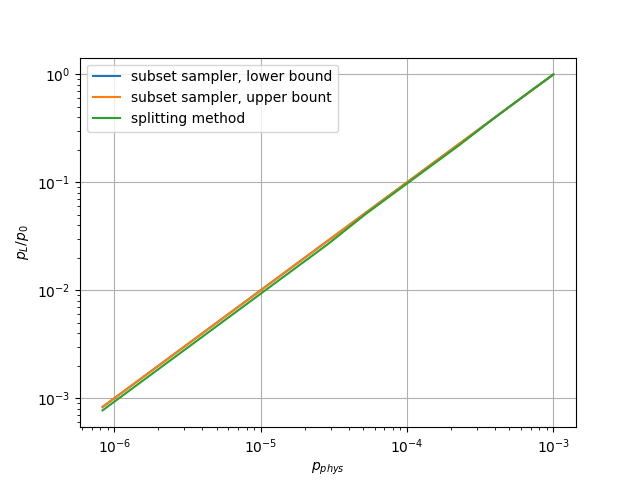
\includegraphics[width=0.8\textwidth]{figs/d11_splitting_vs_qsample.png} 
\caption{Comparison of logical error rates obtained by QSample and the splitting method for distance 11 repetition code.}
\label{fig:d11_vs}
\end{figure}


% Comparison with qsample for distance 3 rotated surface code without any rounds of error correction:

% \begin{figure}[h]
% 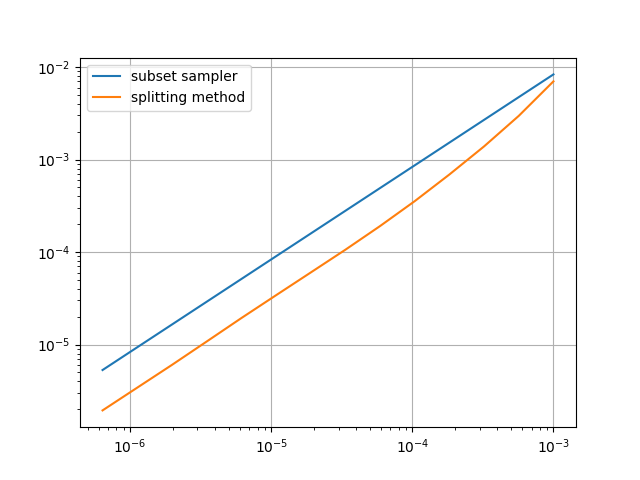
\includegraphics[width=0.8\textwidth, height=6cm]{figs/surface_splitting_vs_qsample.png} 
% \caption{Comparison of logical error rates obtained by QSample and the splitting method for rotated distance 3 surface code.}
% \label{fig:surface}
% \end{figure}

% Comparison with qsample for repetition code for different values of $T_{\mathrm{init}}$:

% \begin{figure}[h]
% 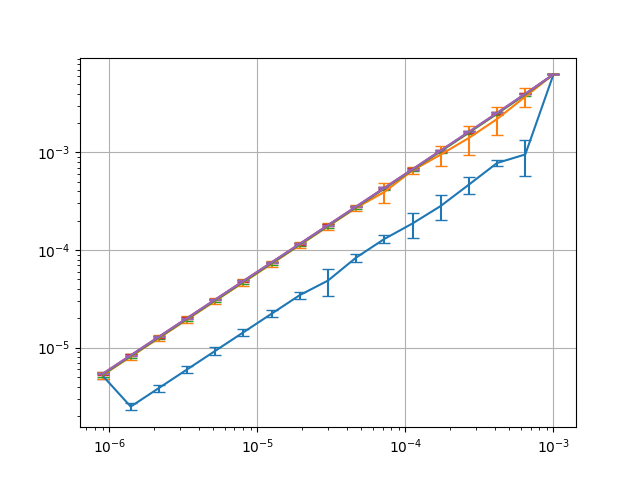
\includegraphics[width=0.8\textwidth, height=6cm]{figs/chain_length_png.png} 
% \caption{Comparison of logical error rates obtained by splitting method for different initial Markov chain lengths.}
% \label{fig:lengths}
% \end{figure}

% \begin{figure}[h]
% 
\includegraphics[width=0.8\textwidth, height=6cm]{figs/repetition_splitting_vs_qsample.png} 
% \caption{Comparison of logical error rates obtained by QSample and the splitting method for repetition code.}
% \label{fig:repetition}
% \end{figure}

% \begin{figure}[h]
% 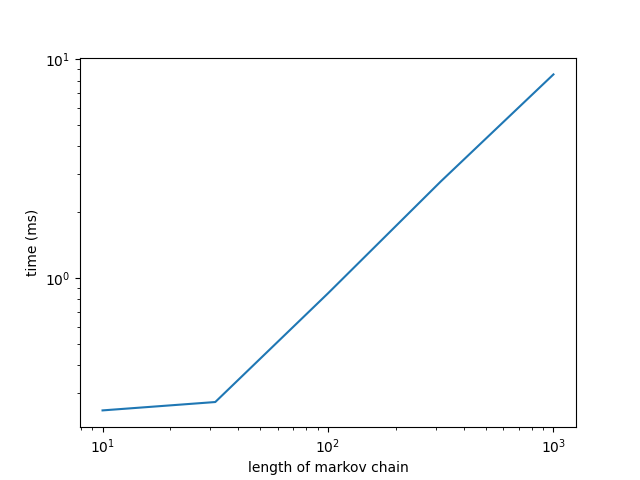
\includegraphics[width=0.8\textwidth, height=6cm]{figs/splitting_times.png} 
% \caption{Computing time of splitting method for different initial Markov chain lengths}
% \label{fig:splitting_times}
% \end{figure}

% \begin{figure}[h]
% 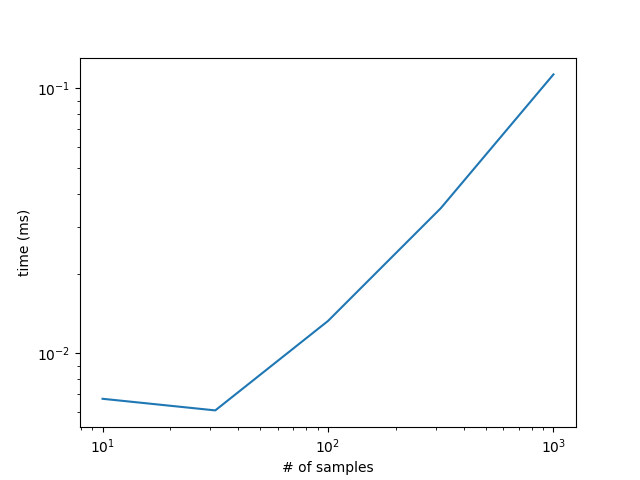
\includegraphics[width=0.8\textwidth, height=6cm]{figs/qsample_times.png} 
% \caption{Computing time of qsample for different numbers of samples}
% \label{fig:qsample_times}
% \end{figure}